% L12b rule-number schematic (November 2026), in the layout of the Fall 2025
% "Two-dimensional Wolfram Totalistic Rules" slide and the style of
% Fig-L12b-RuleSwitch. Each column is one neighbor sum c, from 8 on the left to
% 0 on the right. A column shows one arrangement of four neighbors with that
% sum, the next intention the rule gives, and the place value 3^c. Read from
% left to right, the next intentions are the digits of the rule number.
%
% The digits are decoded here from the rule number, floor(R/3^c) mod 3, so the
% drawing cannot drift from the rule. The notebook SVG gets a dark palette from
% theme_svg.py; add any new color to its mapping.
\documentclass[border=4pt]{standalone}
\usepackage{tikz}
\usepackage{amsmath,amssymb}
\usetikzlibrary{arrows.meta,calc,decorations.pathreplacing}
\definecolor{buyblue}{HTML}{0072B2}
\definecolor{holdgray}{HTML}{AAAAAA}
\definecolor{sellorange}{HTML}{D55E00}
\definecolor{ink}{HTML}{252525}
\newcount\ruledigit
\newcount\rulequotient
\newcount\ruledivisor

\begin{document}
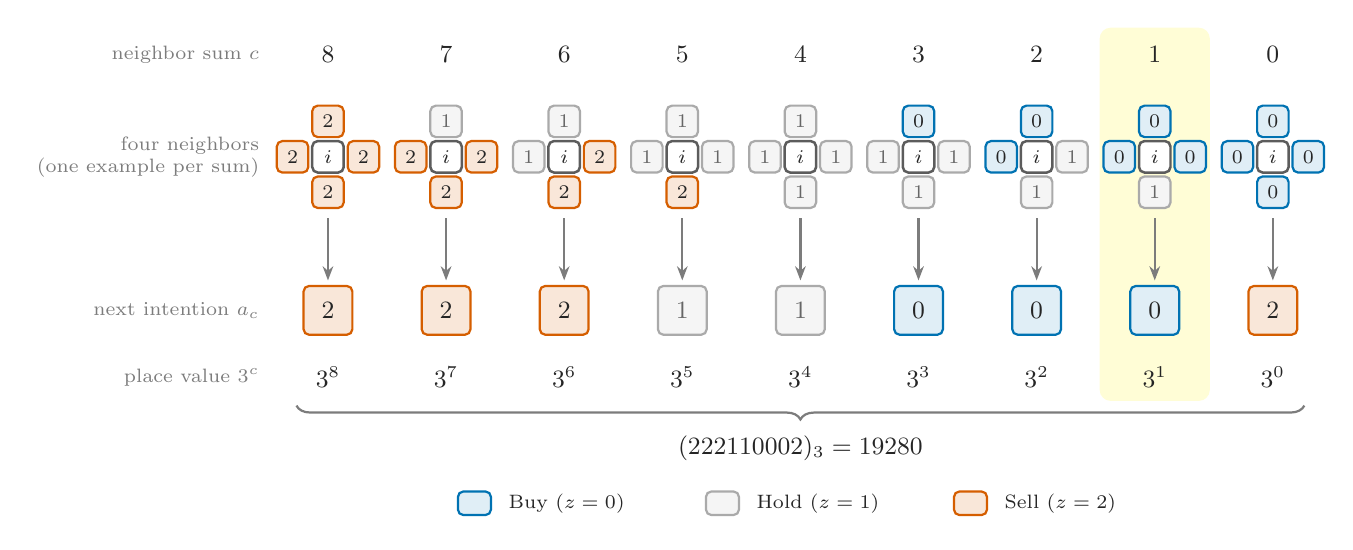
\begin{tikzpicture}[
  x=1cm,y=1cm,
  every node/.style={font=\small,text=ink},
  note/.style={font=\scriptsize,text=ink!60},
  box/.style={rectangle,rounded corners=2pt,thick,inner sep=0pt,align=center},
  buy/.style={box,draw=buyblue,fill=buyblue!12},
  hold/.style={box,draw=holdgray,fill=holdgray!12,text=ink!70},
  sell/.style={box,draw=sellorange,fill=sellorange!15},
  me/.style={box,draw=ink!75,fill=white,line width=.9pt},
  nb/.style={minimum width=.4cm,minimum height=.4cm,font=\scriptsize},
  cell/.style={minimum width=.62cm,minimum height=.62cm},
  arr/.style={-{Stealth[length=1.8mm]},thick,ink!60},
]
\def\rulenumber{19280}
\def\px{1.5}       % column spacing
\def\ns{.45}       % spacing of the tiles in a neighbor cross
\def\ysum{5.45}    % neighbor sum row
\def\ynb{4.15}     % center of the neighbor crosses
\def\ynext{2.2}    % next intention row
\def\yplace{1.35}  % place value row

% ---- band on the column c = 1, the lookup worked in the text ----
\pgfmathsetmacro{\hx}{7*\px}
\fill[yellow!16,rounded corners=4pt] (\hx-.7,\yplace-.3) rectangle (\hx+.7,\ysum+.34);

% ---- row labels ----
\node[note,anchor=east] at (-.75,\ysum) {neighbor sum $c$};
\node[note,anchor=east,align=right] at (-.75,\ynb) {four neighbors\\(one example per sum)};
\node[note,anchor=east] at (-.75,\ynext) {next intention $a_{c}$};
\node[note,anchor=east] at (-.75,\yplace) {place value $3^{c}$};

% ---- one column for each neighbor sum: c / north / west / east / south ----
\foreach \col/\c/\north/\west/\east/\south in {
  0/8/sell/sell/sell/sell,
  1/7/hold/sell/sell/sell,
  2/6/hold/hold/sell/sell,
  3/5/hold/hold/hold/sell,
  4/4/hold/hold/hold/hold,
  5/3/buy/hold/hold/hold,
  6/2/buy/buy/hold/hold,
  7/1/buy/buy/buy/hold,
  8/0/buy/buy/buy/buy} {
  \pgfmathsetmacro{\xc}{\col*\px}
  \node at (\xc,\ysum) {\c};
  % the neighbors, each tile labeled with its intention code
  \foreach \st/\dx/\dy in {\north/0/1,\west/-1/0,\east/1/0,\south/0/-1} {
    \ifnum\pdfstrcmp{\st}{buy}=0 \def\dg{0}\else
      \ifnum\pdfstrcmp{\st}{hold}=0 \def\dg{1}\else \def\dg{2}\fi
    \fi
    \node[\st,nb] at (\xc+\dx*\ns,\ynb+\dy*\ns) {\dg};
  }
  \node[me,nb] at (\xc,\ynb) {$i$};
  \draw[arr] (\xc,\ynb-.78) -- (\xc,\ynext+.38);
  % the digit of this rule at sum c: floor(R/3^c) mod 3
  % TeX integer division avoids PGF's dimension limit for rule IDs >16383.
  \pgfmathtruncatemacro{\power}{pow(3,\c)}
  \ruledivisor=\power\relax
  \ruledigit=\rulenumber\relax
  \divide\ruledigit by \ruledivisor
  \rulequotient=\ruledigit
  \divide\rulequotient by 3
  \multiply\rulequotient by 3
  \advance\ruledigit by -\rulequotient
  \edef\state{\the\ruledigit}
  \ifcase\state
    \node[buy,cell] at (\xc,\ynext) {\state};
  \or
    \node[hold,cell] at (\xc,\ynext) {\state};
  \or
    \node[sell,cell] at (\xc,\ynext) {\state};
  \fi
  \node at (\xc,\yplace) {$3^{\c}$};
}

% ---- the nine digits read as one number ----
\draw[decorate,decoration={brace,mirror,amplitude=5pt},thick,ink!60] (-.4,\yplace-.36) -- (8*\px+.4,\yplace-.36);
\node at (4*\px,\yplace-.9) {$(222110002)_{3}=19280$};

% ---- legend ----
\foreach \xx/\st/\label in {1.65/buy/Buy ($z=0$),4.8/hold/Hold ($z=1$),7.95/sell/Sell ($z=2$)} {
  \node[\st,minimum width=.42cm,minimum height=.3cm] at (\xx+.21,-.25) {};
  \node[note,text=ink,anchor=west] at (\xx+.52,-.25) {\label};
}
\end{tikzpicture}
\end{document}
